Фирма ATMEL --- один из лидеров производства микроконтроллеров. Микроконтроллеры ATmega в большинстве своём работают на частоте 16 МГц. Это означает, что одна инструкция программы выполняется за 1/16000000 секунды, т. е. выполняется 16 миллионов инструкций за 1 секунду. Блок-схема ATmega328 показана на рисунке~\ref{fig:atmegablock}~\cite{atmega:328}.

\begin{figure}[ht]
    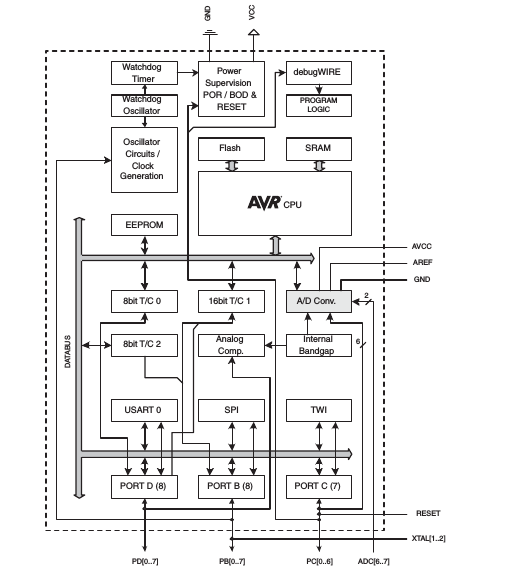
\includegraphics[width=.6\linewidth]{Figures/atmegablock.png}
    \caption{Блок-схема ATmega328}
    \label{fig:atmegablock}
\end{figure}
